\section{Partie graphique}


\subsection{Coté interface utilisateur}
\subsubsection{MaterializeCSS}
Pour l'interface utilisateur, nous avons dû utiliser la bibliothèque graphique \href{http://www.materializecss.com/}{{\it MaterializeCSS}} qui fournit un dossier compressé comprenant tous les fichiers de base d'un site web. Ceci permet d'avoir une architecture de fichiers déjà existante et fournir les fichiers CSS nécessaires pour avoir un visuel optimisé et un design attirant.

Ainsi, il suffit d'appeler un élément graphique de HTML, de lui donner la classe correspondante implémentée dans {\it MaterializeCSS} et le visuel est prêt.

%%
\subsubsection{Structure du site}

Le site est en {\it monopage}, c'est à dire qu'il n'y a pas de présence de plusieurs fichiers HTML à charger ou d'un serveur avec une base de données pour les différents élements.

Pour passer d'un contenu à un autre, nous utilisons l'élément HTML de navigation. Ainsi, cela donne l'effet de trois pages: \textbf{Acceuil}, \textbf{Commencer} et \textbf{À Propos}, alors qu'il ne s'agit que d'un seul fichier HTML.\\

Dans la partie \textbf{Commencer}, nous pouvons séparer cette partie en trois sous-catégories. La première permet à l'utilisateur de saisir ces paramètres (les fichiers de données, ses fonctions map/reduce et les paramètres du cluster).
La seconde permet soit d'écrire les fonctions map/reduce directement sur le site, ou de visualiser le code fournis pour le corriger directement.
Enfin la dernière section concerne la simulation avec {\it FATuM} pour le cluster et une colonne à droite de la page pour l'affichage des données contenues dans un slot.

\subsubsection{Les Loaders}
\begin{figure}[H]
  \centering
    
\includegraphics[scale=0.5]{images/loader.png}
        \caption{Loader}
        \label{fig:loader}
\end{figure}
Le temps de chargement du site au démarrage ainsi que lors du lancement de la simulation est long. Cette lenteur peut être interprétée par le temps que met \textit{FATuM} pour se charger. C'est pourquoi nous avons visé à rajouter un "Loader" (voir Figure \ref{fig:loader}) au démarrage de la page (pour signifier le chargement de \textit{FATuM}) et un autre pour le temps de calcul de la simulation. Le loader du démarrage fonctionne. Malheureusement, celui de la simulation n'a pas pu être implémenté. En effet, le site se bloque le temps de calcul ce qui empêche l'utilisation du loader.

\newpage
\subsubsection{Les paramètres}
Les {\tt paramètres} entrés par l'utilisateur doivent remplir certaines conditions. En voici une liste exhaustive.
\begin{itemize}
\item Le cluster du Map doit avoir un nombre de machines compris entre 1 et 20 PCs et un nombre de coeurs compris entre 1 et 24. \\ Cette limitation est due à l'inconfort visuel que peut apporter un très grand cluster. En effet, au delà de ces valeurs, la lisibilité n'est plus assurée. Il s'agit là, d'un choix par le groupe suite aux conseils du client.
\item Le nombre de {\tt reduce()} doit être compris entre 1 et le nombre de slots total du cluster de {\tt map()}.
\item Il n'est pas nécessaire d'importer un fichier {\tt .js} pour les fonctions mapReduce. L'utilisateur peut directement coder  dans la "section code". Nous avons aussi fournit un exemple de code qui est fonctionnel et qui implémente l'exemple de WordCount (comme vu dans la figure 1.2 du premier chapitre).
\item Le fichier csv doit être impérativement fourni.
Si l'utilisateur rafraîchit la page, le contenu du fichier disparaît même si le nom du fichier reste, il faut donc la charger de nouveau.
\end{itemize}


\subsection{Simulation graphique(Fatum)}
Comme demandé par le client, nous avons utilisé la bibliothèque graphique \href{http://www.labri.fr/perso/aperrot/fatum/index.html}{{\it FATuM}} développée au \href{http://www.labri.fr/}{{\it LaBRI}}. Cette bibliothèque permet d'afficher la simulation du cluster (voir Figure \ref{fig:sim}) avec différents composants graphiques et ne peut être utilisée pour l'interface utilisateur contrairement à \textit{MaterializeCSS}.
%image fatum simple avec connection.
\begin{figure}[H]
  \centering
    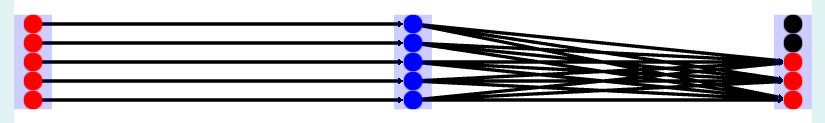
\includegraphics[scale=0.45]{images/graphiqueExemple.png}
        \caption{FATuM - Simulation}
        \label{fig:sim}
\end{figure}

Nous utilisons plusieurs composants de FATuM:
\begin{itemize}
\item Les Marks
\item Les Connections
\item Le zoom
\item Une partie de la gestion d'un "clic souris"\\
\end{itemize}

\begin{figure}[H]
  \centering
    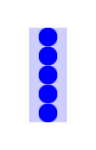
\includegraphics[scale=0.5]{images/marks.png}
        \caption{FATuM : Marks}
        \label{fig:mark}
\end{figure}
Un {\it Mark} (comme dans la figure \ref{fig:mark}) est un élément sous forme de cercle qui représente un slot du cluster. Ils sont séparés entre eux lorsque la limite de slots par PC est atteinte. Ainsi, chaque PC sont séparés graphiquement. Ces éléments graphiques sont dépendants des données fournies par l'utilisateur.\\

Les {\it connections} sont les flèches qui vont d'un Mark vers un autre. Ils représentent le transfert de données entre les slots. On trouve des connections entre l'input de map et map ainsi que des connections entre map et reduce.\\

Le {\it zoom} permet (si l'on pose le pointeur de la souris dans la zone de simulation gérée par \textit{FATuM}) la gestion de la molette de la souris. Ainsi, en cas d'un gros cluster, l'ensemble reste lisible grâce à ce zoom. \\

Enfin, la gestion du {\it clic souris}. Lors d'un clic dans la zone de simulation \textit{FATuM}, les coordonnées récupérées sont celles de la fenêtre. Elles n'ont donc rien à voir avec celles de \textit{FATuM}. La fonction {\tt windowToModel} nous a permis de transformer les coordonnées du clic en coordonnées compréhensibles par \textit{FATuM} pour pouvoir exécuter le traitement suivant la zone de clic.


\subsubsection{Précision sur la fonction "search\_mark"}

\begin{lstlisting}
function search_mark(x, id) {
    var header_data, tmp_header;
    //type of the mark
    switch (x) {
        case indice_fatum_1:
            tmp_header = "Map Input--";
            break;

        case indice_fatum_2:
            tmp_header = "Map Output--";
            break;

        case indice_fatum_3:
            tmp_header = "Reduce Output--";
            break;
        default:
            return false;
    }
    var min = nb_slot + gap;
    var max = min + nb_slot;
    //researh the true id without the gap
    for (var i = 0; i < nb_pc; i++) {
        if (0 <= id && id < nb_slot) {
            header_data = "Slot " + id + ": --"; //exple: Slot 1: --Map Task--
            print_data(x, id, header_data + tmp_header);
            break;
        } else
        if (min <= id) {
            if (id < max) {
                id = id - (gap * (i + 1));
                header_data = "Slot " + id + ": --";
                print_data(x, id, header_data + tmp_header);
                break;
            }
        }
        min = max + gap;
        max = min + nb_slot;
    }
}
\end{lstlisting}
\newpage
Cette fonction nécessite des précisions. 

En effet, pour différencier les blocs de PCs, nous mettons un décalage (variable \textbf{gap}) entre ces blocs. Ce décalage crée des erreurs d'id de mark par la suite. En effet, lorsque l'on clique sur un slot, son id correspond à sa position dans l'axe des y. Mais à cause de ce décalage, l'espacement est également considéré comme un bloc et les id sont décalés. Il serait donc possible, par exemple, de cliquer dans une zone \textit{vide} entre deux machines et ce clic considère que c'est un id valide.\\

D'autre part, cette fonction permet de détecter quel type de donnée on souhaite afficher (map input, map output ou reduce output). Pour cela, on utilise l'axe des X pour se repérer. A titre d'exemple, un clic qui a en x une valeur correspondant à "indice\_fatum\_1" vaut toute la colonne des slots des map inputs.

\subsubsection{La sortie console}
Lors du démarrage de l'application, l'initialisation de \textit{FATuM} s'effectue. Il est donc normal de voir en console (comme dans la figure \ref{fig:console}) des informations concernant la bibliothèque.

\begin{figure}[H]
  \centering
    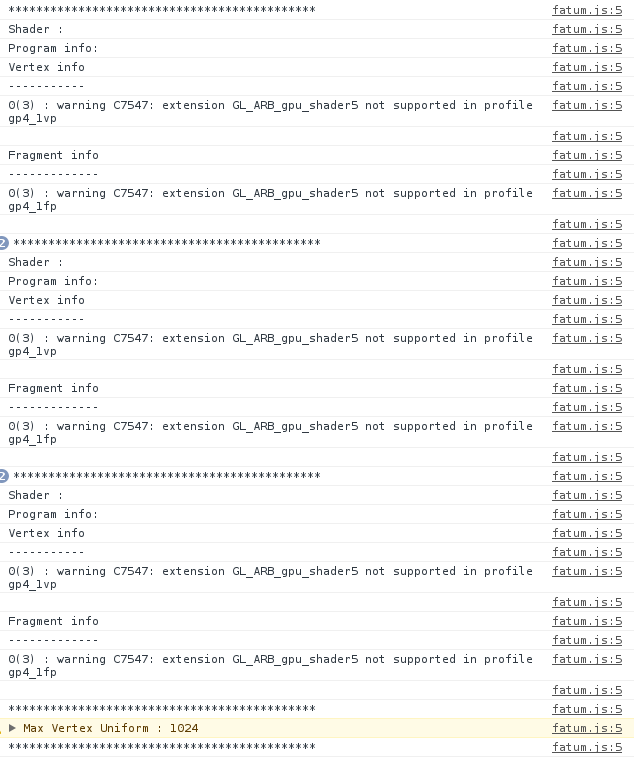
\includegraphics[scale=0.5]{images/console_fatum.png}
        \caption{Sortie console de l'initialisation de \textit{FATuM}}
        \label{fig:console}
\end{figure}

